\documentclass[conference]{IEEEtran}
\IEEEoverridecommandlockouts

\usepackage[utf8]{inputenc}
\usepackage[T1]{fontenc}
\usepackage{amsmath,amssymb}
\usepackage{graphicx}
\usepackage{booktabs}
\usepackage{multirow}
\usepackage{array}
\usepackage{xcolor}
\usepackage{url}
\usepackage{cite}
\usepackage{tikz}
\usetikzlibrary{positioning,arrows.meta,fit}
\graphicspath{{figures/}}

\begin{document}

\title{ShopSense AI: A Student-Focused Shopping Platform with Hybrid Recommendations, Semantic Search and Review Intelligence}

% Replace the bracketed placeholders with your college details before submitting.
\author{
\IEEEauthorblockN{Aanchal Yadav}
\IEEEauthorblockA{\textit{Dept. of Computer Science and Engineering}\\
\textit{[College Name]}\\
[City], India}
\and
\IEEEauthorblockN{Riya Aryan}
\IEEEauthorblockA{\textit{Dept. of Computer Science and Engineering}\\
\textit{[College Name]}\\
[City], India}
\and
\IEEEauthorblockN{Susmita}
\IEEEauthorblockA{\textit{Dept. of Computer Science and Engineering}\\
\textit{[College Name]}\\
[City], India}
\and
\IEEEauthorblockN{Sneha}
\IEEEauthorblockA{\textit{Dept. of Computer Science and Engineering}\\
\textit{[College Name]}\\
[City], India}
}

\maketitle

\begin{abstract}
Students buying things for college (a first laptop, a calculator for an engineering exam, a kettle for the hostel room) often know what they need but not what the product is called. Typical e-commerce search expects exact keywords, and new users get generic suggestions because the site knows nothing about them yet. We built ShopSense AI, a web platform for this audience that combines several recommendation approaches with natural language processing. Four models contribute recommendations: a content-based model using TF-IDF with fuzzy, adaptive interaction weights; an SVD collaborative filter; a Neural Collaborative Filtering (NeuMF) model; and a survey-based model in which a new user's answers are written out as a sentence and matched against products using sentence embeddings. A gateway blends these signals and explains each suggestion. On the language side, the platform offers semantic search with MiniLM embeddings and a FAISS index, review analysis with VADER sentiment and TF-IDF theme extraction, and a chatbot that can search, recommend, compare products and summarise reviews. In our tests, semantic search answered in about 15--21\,ms at the 95th percentile, the intended product appeared in the top three for all 15 natural-language test queries, and the chatbot classified all 30 labelled test messages correctly. We also discuss the limits of our evaluation, mainly the small catalogue and the synthetic review data.
\end{abstract}

\begin{IEEEkeywords}
recommender systems, neural collaborative filtering, semantic search, sentiment analysis, conversational agents, cold start
\end{IEEEkeywords}

%--------------------------------------------------------------------
\section{Introduction}
Most of us have searched a shopping site for something like ``a bottle that keeps tea hot'' and got results for tea bags. Keyword search works well when you already know the product name, and much less well when you only know the problem you are trying to solve. Students are a good example of this. They are often buying a category of product for the first time, they work to tight budgets, and their needs are tied to situations such as online classes, coding assignments or living in a hostel.

A second problem appears on the first visit. Recommendation engines learn from clicks and purchases, so a new user with no history usually sees a list of best-sellers, which may have little to do with what they need. This is the well-known cold-start problem~\cite{schein2002}.

A third problem is reviews. Popular products can have hundreds of them, and few people read more than a handful before deciding.

ShopSense AI tries to address all three. It is a full-stack web application with a React frontend, a Flask backend and separate services for recommendation and language processing. The work was split among four team members: the frontend and content-based model; the backend and collaborative filtering; the deep-learning recommender and hybrid engine; and the NLP service with the chatbot and survey. This paper describes how the pieces fit together, what each model does, and how well the system performed in our tests.

%--------------------------------------------------------------------
\section{Related Work}
Content-based recommenders describe items by their features and suggest items similar to those a user liked before~\cite{lops2011}. They handle new items well but tend to keep suggesting more of the same. Collaborative filtering instead learns from the behaviour of many users. Matrix factorisation methods such as SVD became widely used after the Netflix Prize~\cite{koren2009}. He~\textit{et al.}~\cite{he2017} showed that replacing the inner product with a neural network (Neural Collaborative Filtering) can capture non-linear user--item interactions. Hybrid systems combine several of these approaches to offset their individual weaknesses~\cite{burke2002}.

For search, Sentence-BERT~\cite{reimers2019} made it practical to compare short texts by meaning, and libraries such as FAISS~\cite{johnson2019} make nearest-neighbour lookup over the resulting vectors fast. For review analysis, VADER~\cite{hutto2014} is a rule-based sentiment model that needs no training data and runs quickly, while transformer models such as DistilBERT~\cite{sanh2019} are more expressive but heavier. Fuzzy logic~\cite{zadeh1965} has also been used to soften fixed thresholds and weights in recommenders. Our contribution is mostly in combining these known techniques around a student use case, and in using the same embedding space for both search and survey-based cold-start recommendations.

%--------------------------------------------------------------------
\section{Objectives}
We set the following goals at the start of the project:
\begin{enumerate}
\item Recommend products that match a student's needs, budget and behaviour, including on their very first visit.
\item Let users search in plain language instead of exact keywords.
\item Summarise customer reviews into a sentiment score and a short list of what people like and dislike.
\item Provide a chatbot that can find, recommend and compare products and answer questions about reviews.
\item Compare the individual recommendation models and the hybrid on standard ranking metrics.
\end{enumerate}

%--------------------------------------------------------------------
\section{System Architecture}
Fig.~\ref{fig:arch} shows the overall design. The React single-page application talks only to the Flask backend, which acts as a gateway. The backend owns the database (users, products, reviews, interactions, cart, wishlist and survey answers) and forwards AI requests to the services behind it: the content-based and SVD service, the NCF hybrid service, and the NLP service. Every call to an AI service has a short timeout and a fallback. If the NLP service is down, for example, semantic search falls back to keyword search instead of failing.

\begin{figure}[t]
\centering
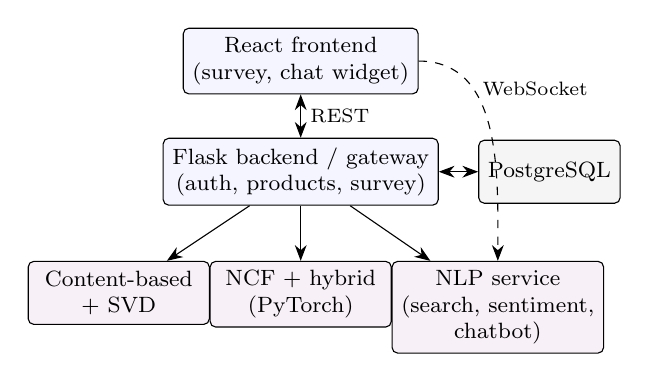
\begin{tikzpicture}[
  box/.style={draw, rounded corners=2pt, align=center, font=\footnotesize, minimum width=2.3cm, minimum height=0.8cm, fill=blue!4},
  svc/.style={box, fill=violet!6},
  >={Stealth[length=2mm]}]
\node[box] (fe) {React frontend\\(survey, chat widget)};
\node[box, below=0.55cm of fe] (be) {Flask backend / gateway\\(auth, products, survey)};
\node[svc, below left=0.7cm and -0.6cm of be] (cb) {Content-based\\+ SVD};
\node[svc, below=0.7cm of be] (ncf) {NCF + hybrid\\(PyTorch)};
\node[svc, below right=0.7cm and -0.6cm of be] (nlp) {NLP service\\(search, sentiment,\\chatbot)};
\node[box, right=0.5cm of be, fill=gray!8, minimum width=1.6cm] (db) {PostgreSQL};
\draw[<->] (fe) -- node[right, font=\scriptsize]{REST} (be);
\draw[->] (be) -- (cb);
\draw[->] (be) -- (ncf);
\draw[->] (be) -- (nlp);
\draw[<->] (be) -- (db);
\draw[->, dashed] (fe.east) to[out=0, in=90] node[right, font=\scriptsize, pos=0.3]{WebSocket} (nlp.north);
\end{tikzpicture}
\caption{High-level architecture. The chatbot uses a WebSocket directly to the NLP service; everything else goes through the backend gateway.}
\label{fig:arch}
\end{figure}

%--------------------------------------------------------------------
\section{Methodology}

\subsection{Data}
The catalogue has 20 real products in nine student-oriented categories: laptops, tablets, smartphones, audio, computer accessories, study essentials, hostel essentials, backpacks, and storage. Each product has a description, specifications and links to marketplaces. Since we had no real customer reviews for these exact products, we generated 240 \emph{synthetic} reviews (12 per product) from product-specific phrases about real strengths and weaknesses, such as soldered RAM on one laptop or expensive ink on the printer. Star ratings were drawn from a per-product distribution and the text was written to match the rating, with deliberately mixed 3-star reviews. Four demo users with different personas and 16 reviewer accounts produce 502 interaction events (view, click, wishlist, cart and purchase). We state this clearly because it limits how far our sentiment results can be generalised.

\subsection{Content-Based Model with Fuzzy Weights}
Each product is represented by a TF-IDF vector over its name, description, category and a set of keywords. A user's profile is the weighted average of the vectors of the products they interacted with. Instead of fixed weights per event type, the weights adapt to the user: the frequency of each event type is mapped to low, medium and high fuzzy memberships, defuzzified, and used to adjust the base weight by at most 10\%. The adjustment is scaled by a confidence term $n/(n+10)$, where $n$ is the number of interactions. The final score combines profile similarity (65\%) with item-to-item similarity (35\%), excludes items already bought or in the cart, and caps any single category at three results to keep some variety.

\subsection{Collaborative Filtering (SVD)}
Interactions are converted to implicit ratings from 1 to 5 (view = 1 up to purchase = 5, summed and capped) to form a user--item matrix. Our first version used a truncated NumPy SVD with $k = 2$ latent factors. The final version uses the SVD implementation in the Surprise library (10 factors, 40 epochs), which learns user and item biases and only fits the observed ratings. Unseen items are ranked by their predicted rating, and new users fall back to a popularity ranking.

\subsection{Neural Collaborative Filtering}
The NeuMF model~\cite{he2017} has two branches. The GMF branch takes the element-wise product of 32-dimensional user and item embeddings. The MLP branch concatenates separate embeddings and passes them through layers of 64, 32 and 16 units with ReLU. Both outputs are concatenated and fed to a sigmoid output. Training uses binary cross-entropy, with four sampled negatives per positive and the Adam optimiser (learning rate 0.001) for 20 epochs. We keep the checkpoint with the lowest training loss.

\subsection{Hybrid Engine and Recommendation Gateway}
The hybrid engine min--max normalises the three model scores and combines them as
\begin{equation}
s_{\text{hybrid}} = 0.3\,s_{\text{SVD}} + 0.3\,s_{\text{CB}} + 0.4\,s_{\text{NCF}}.
\end{equation}
The backend gateway then blends whichever signals exist for the current user (hybrid, content-based history, survey and popularity), weighting them 0.45, 0.30, 0.35 and 0.10 and renormalising over the sources that are available. Each recommendation keeps the source that contributed most to it, which becomes the explanation shown to the user, such as ``Similar to products you've interacted with'' or ``Matches your interest in Laptops''.

\subsection{Semantic Search}
For every product we join the name, brand, category, description and specifications, clean the text, and encode it with all-MiniLM-L6-v2~\cite{reimers2019} into a 384-dimensional unit vector. The vectors go into a FAISS \texttt{IndexFlatIP} index~\cite{johnson2019}, where the inner product equals cosine similarity. A query is encoded the same way and the closest products are returned, with optional price and category filters. The index is saved with a fingerprint of the catalogue and is rebuilt only when products change.

\subsection{Sentiment Analysis and Review Summaries}
Each review is scored with VADER~\cite{hutto2014}. A compound score above 0.05 counts as positive, below $-0.05$ as negative, and anything in between as neutral. VADER was built for social media text and misses many product-specific complaint words such as ``expensive'', ``lags'' and ``leaks'', so we added a small e-commerce lexicon of about 70 words at 0.7 of their base weight. We left out context-dependent words such as ``hot'' (as in ``keeps tea hot''). For each product we count the sentiment classes and extract themes with TF-IDF over phrases of adjacent words, ranking a phrase by how much more often it appears on one side (positive or negative) than the other. This produces themes such as ``ink cartridges'' for the printer and ``headband cracked'' for one of the headphones, along with a one-sentence verdict.

\subsection{Conversational Assistant}
The chatbot uses a rule-based intent router with seven intents: greeting, help, search, recommendation, comparison, review summary and product information, plus a fallback. Alongside the intent it extracts products, budgets and categories. Product names are matched by weighting each word of the name by how identifying it is: a model number unique to one product (``CH520'', ``A9'') counts much more than a shared word like ``headphones''. Budgets such as ``under 5k'' or ``between 2000 and 4000'' are parsed with regular expressions. The bot remembers the products from its last answer, so follow-ups like ``what do people think about it?'' or ``compare them'' work as expected. Responses are structured JSON, so the frontend can show product cards, comparison tables and sentiment bars instead of plain text. Messages travel over Flask-SocketIO, with a REST fallback.

\subsection{Preference Survey for Cold Start}
New users can fill in a five-step survey covering their role, categories of interest, intended use, budget, priorities, preferred brands and an optional free-text description. The answers are turned into a short need statement, for example ``I am a college undergraduate student. I will use it for hostel room living\ldots'', which is embedded in the same space as the products. Each product then receives
\begin{equation}
\begin{split}
s = {}& 0.40\,s_{\text{sem}} + 0.25\,s_{\text{cat}} + 0.20\,s_{\text{budget}}\\
& + 0.10\,s_{\text{sent}} + 0.05\,s_{\text{brand}},
\end{split}
\end{equation}
where $s_{\text{budget}}$ falls off smoothly as $(B/p)^2$ for items priced $p$ above the budget $B$, and $s_{\text{sent}}$ is the share of positive reviews. The result page shows a match percentage and the reasons behind each pick.

%--------------------------------------------------------------------
\section{Implementation}
The frontend uses React with Vite and Tailwind CSS. The backend uses Flask with SQLAlchemy, Flask-JWT-Extended and PostgreSQL. The recommendation models use scikit-learn, NumPy and PyTorch, and the hybrid is served with FastAPI. The NLP service uses sentence-transformers, FAISS, vaderSentiment and Flask-SocketIO. Personal recommendations are cached for an hour under the key \texttt{user:\{id\}:recs} (in Redis when available) and invalidated whenever the user changes their cart, wishlist, survey or interaction history. The schema is managed with Alembic migrations. A Docker Compose file starts the whole stack. For a lightweight hosted demo we also run the backend, recommender and NLP code inside a single serverless function on Vercel; this version uses TF-IDF vectors and REST chat because the transformer model exceeds the platform's size limit. The project has 106 automated tests across the backend and the NLP service.

%--------------------------------------------------------------------
\section{Results}

\subsection{Search, Sentiment and Chatbot}
Table~\ref{tab:nlp} summarises the NLP benchmarks, run on a laptop CPU. Search latency is far below our 200\,ms target. For relevance, we wrote 15 queries that describe a need rather than name a product, such as ``something to keep my tea hot during lectures'' and ``solve matrices in the engineering exam''. In every case the intended product was among the top three results, and in most cases it was first.

\begin{table}[t]
\caption{NLP Service Benchmarks}
\label{tab:nlp}
\centering
\begin{tabular}{@{}lr@{}}
\toprule
Metric & Result \\
\midrule
Search latency, mean / p95 (60 queries) & 13--14 / 15--21 ms \\
Relevance: hit rate@3 (15 queries) & 15/15 \\
Intent accuracy (30 labelled messages) & 30/30 \\
\bottomrule
\end{tabular}
\end{table}

Table~\ref{tab:sent} compares sentiment models on a random sample of 100 reviews, with star ratings as ground truth (4--5 positive, 3 neutral, 1--2 negative). Plain VADER did slightly better on this sample, and the two VADER variants tied at 81\% over all 240 reviews. We kept the domain lexicon because it fixes product-level verdicts: without it, VADER labelled 8 of the printer's 12 reviews positive even though the average rating was 3 stars. DistilBERT fine-tuned on SST-2 scored poorly, mostly because it only predicts two classes and our reviews are often mixed. The neutral class is the weak spot for every model, since a 3-star review that praises one thing and criticises another rarely reads as neutral.

\begin{table}[t]
\caption{Sentiment Accuracy Against Star Ratings (100 Reviews)}
\label{tab:sent}
\centering
\begin{tabular}{@{}lccc@{}}
\toprule
Model & 3-class & Pos.\ vs.\ neg. & ms/review \\
\midrule
VADER & 85\% & 93\% & 0.1 \\
VADER + domain lexicon & 82\% & 91\% & 0.1 \\
DistilBERT (SST-2) & 56\% & 63\% & 24 \\
\bottomrule
\end{tabular}
\end{table}

\subsection{Recommendation Models}
For rating prediction on a timestamp split (80/20 per user), Surprise SVD reached an RMSE of 0.53 and MAE of 0.17, against 2.94 and 2.64 for the first NumPy version. The NumPy version treated every unobserved entry as zero, which pulled its predictions down.

To compare all five approaches on equal terms, we ran a leave-one-out evaluation over the 19 users with at least two products. Each user's most recent product was held out and ranked against the products they had not touched (7.7 candidates on average); ties counted against the model. Table~\ref{tab:rec} and Fig.~\ref{fig:models} show the results. Content-based filtering gave the best NDCG@10 and MRR, and NCF the best hit rate. The hybrid came close to the best single models but did not beat them, even after we tuned its weights by grid search on a separate validation split, which moved weight from SVD to the content model. We think the reason is the data: the reviewer histories are random, so there is little collaborative signal for the hybrid to add, and with only 20 products a single position in the ranking changes the metrics noticeably. We report this as it is rather than tuning on the test set.

\begin{table}[t]
\caption{Leave-One-Out Comparison (19 Users)}
\label{tab:rec}
\centering
\begin{tabular}{@{}lccc@{}}
\toprule
Model & HR@10 & NDCG@10 & MRR \
\midrule
Popularity & 0.947 & 0.373 & 0.204 \
SVD (Surprise) & 0.947 & 0.412 & 0.250 \
Content-based (TF-IDF) & 0.947 & \textbf{0.576} & \textbf{0.465} \
NCF (NeuMF) & \textbf{1.000} & 0.569 & 0.434 \
Hybrid (0.3 / 0.3 / 0.4) & 0.895 & 0.559 & 0.460 \
Hybrid, tuned (0.1 / 0.5 / 0.4) & 0.895 & 0.557 & 0.458 \
\bottomrule
\end{tabular}
\end{table}

\begin{figure}[t]
\centering
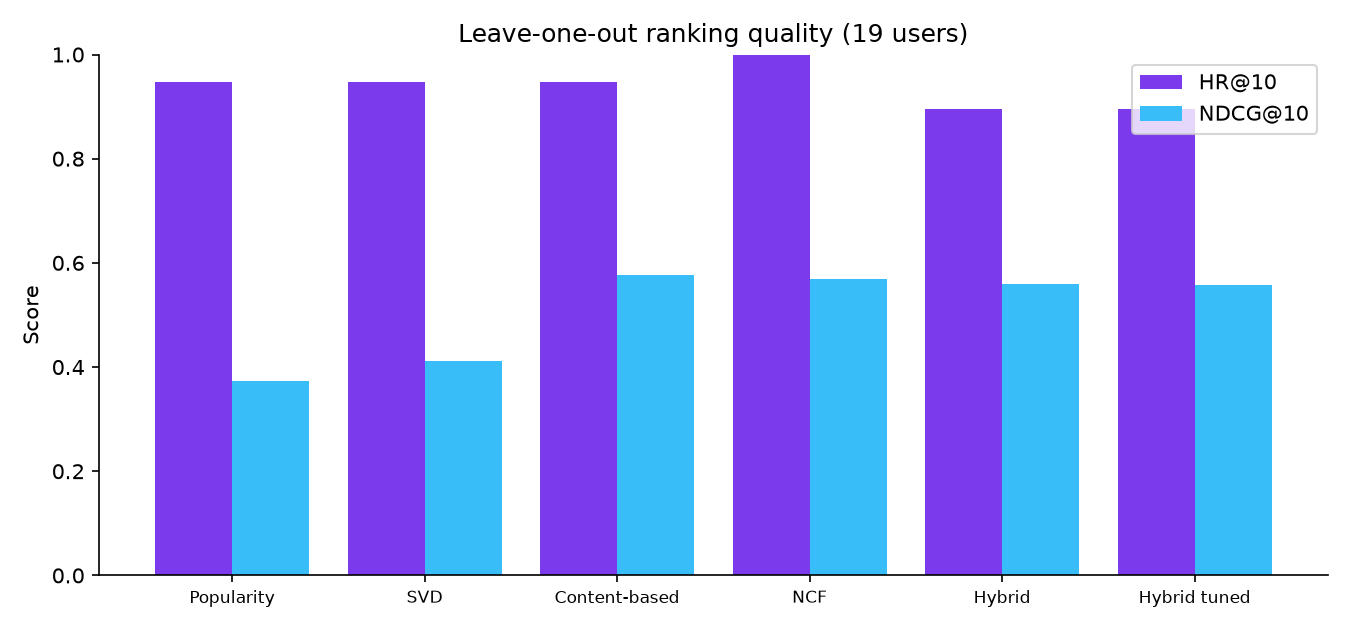
\includegraphics[width=\linewidth]{hr_ndcg_by_model.png}
\caption{HR@10 and NDCG@10 for each recommendation model.}
\label{fig:models}
\end{figure}

\subsection{User Interface}
Figs.~\ref{fig:search}--\ref{fig:chat} show the system in use. The survey (Fig.~\ref{fig:survey}) gave sensible results for a hostel-living persona with a Rs.~3,000 budget: backpacks, a thermos bottle, the kettle and a power extender ranked at the top, each with a reason attached.

\begin{figure}[t]
\centering
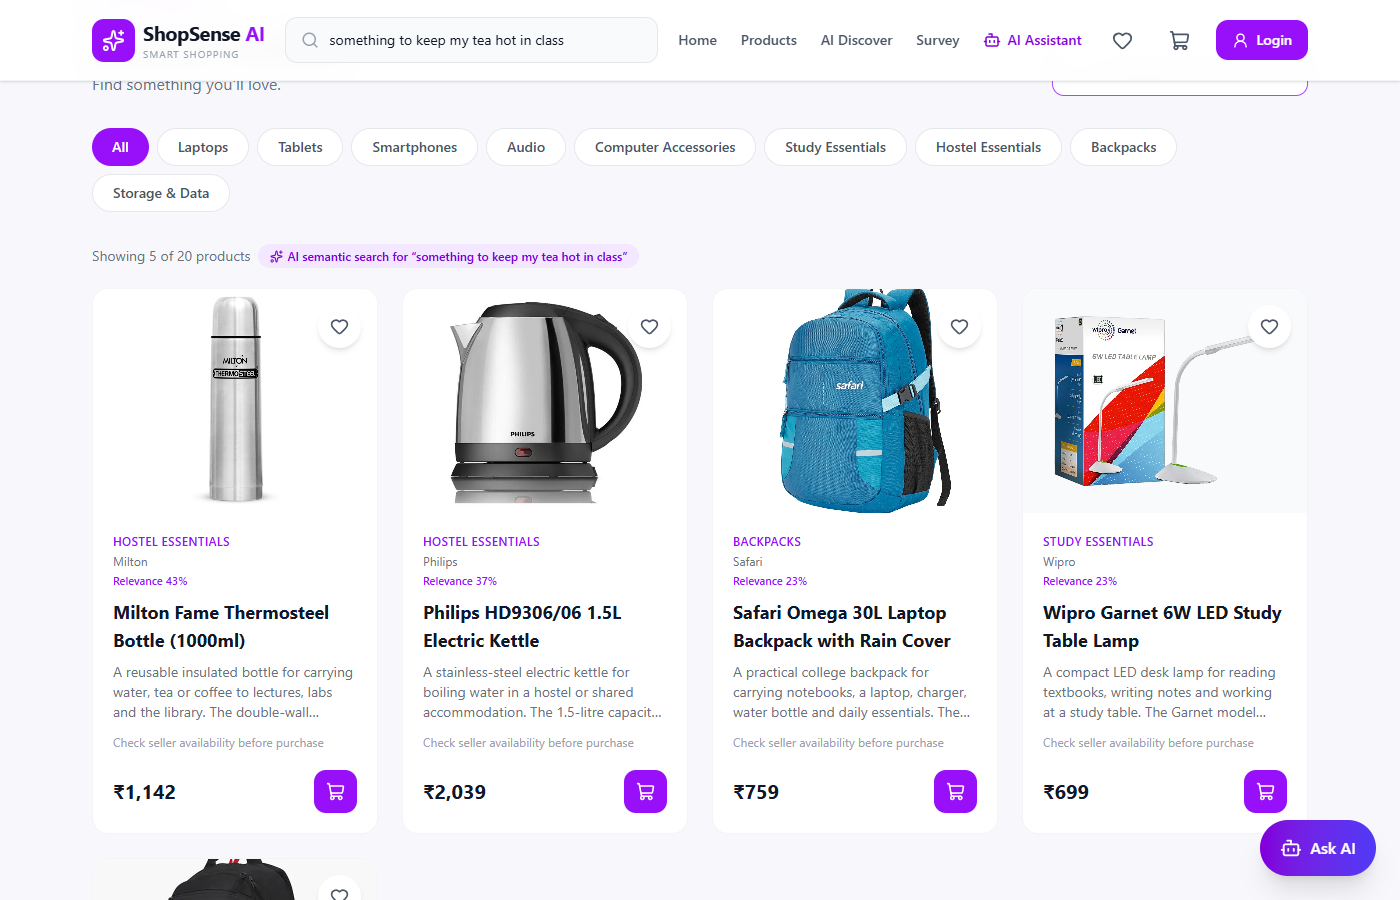
\includegraphics[width=\linewidth]{02_semantic_search.png}
\caption{Semantic search for ``something to keep my tea hot in class'': the insulated bottle and the kettle rank first.}
\label{fig:search}
\end{figure}

\begin{figure}[t]
\centering
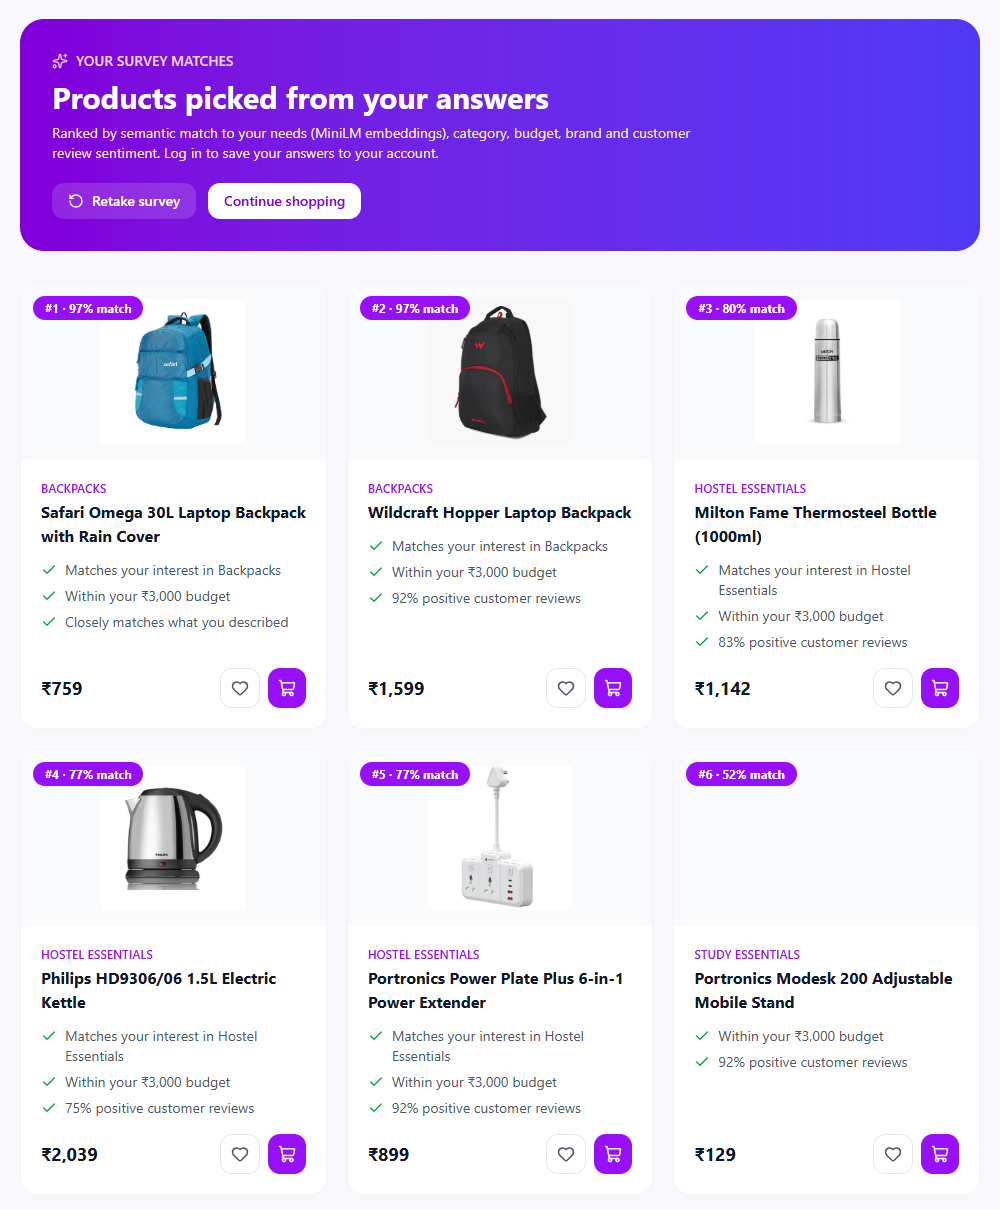
\includegraphics[width=\linewidth]{03c_survey_results.png}
\caption{Survey results for a hostel student with a Rs.~3,000 budget, with match scores and reasons.}
\label{fig:survey}
\end{figure}

\begin{figure}[t]
\centering
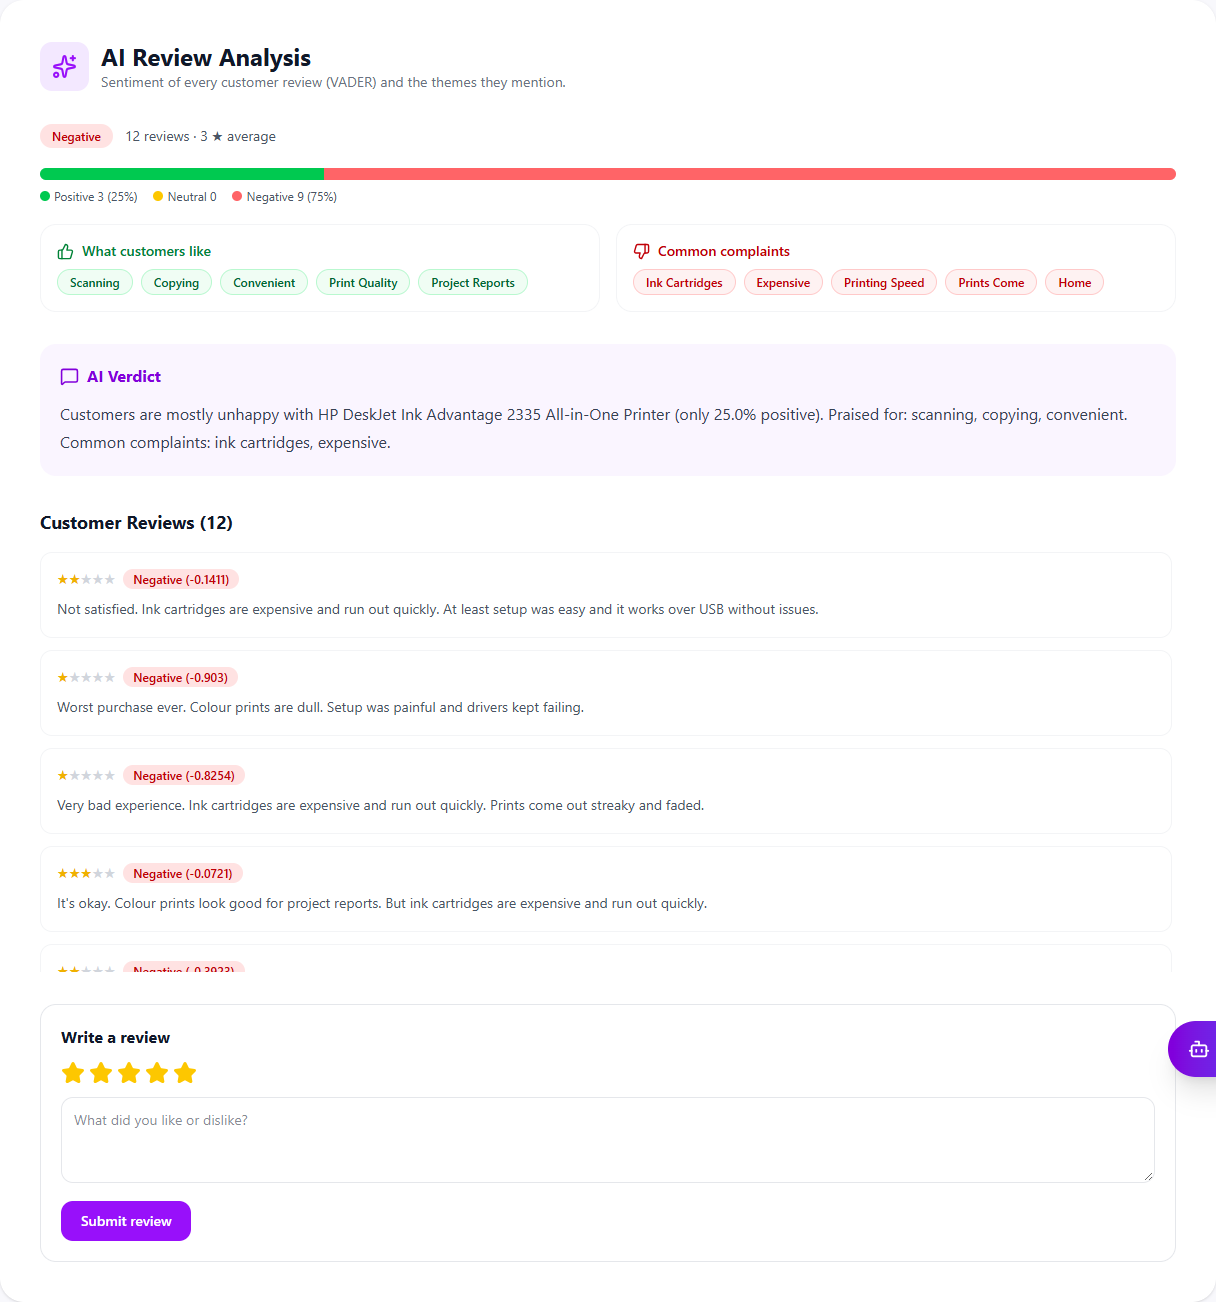
\includegraphics[width=\linewidth]{05_product_review_analysis.png}
\caption{Review analysis for the printer: sentiment split, praise and complaint themes, verdict and per-review labels.}
\label{fig:reviews}
\end{figure}

\begin{figure}[t]
\centering
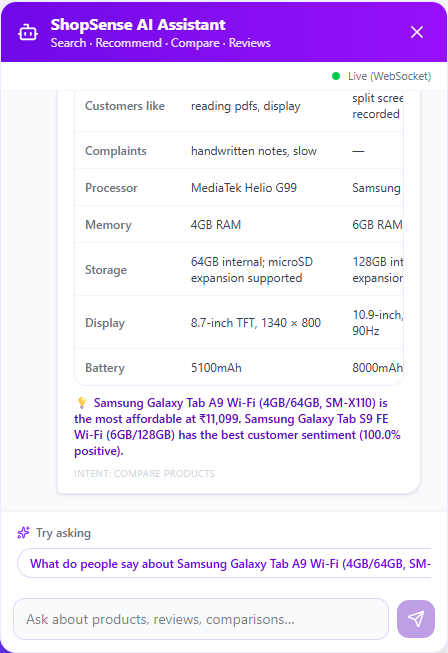
\includegraphics[width=0.62\linewidth]{06b_chat_compare.png}
\caption{The chatbot comparing two tablets side by side.}
\label{fig:chat}
\end{figure}

%--------------------------------------------------------------------
\section{Limitations}
The biggest limitation is the data. The reviews are synthetic, so the sentiment numbers show that the pipeline works rather than how accurate it would be on real customer text, and we tuned the domain lexicon on the same reviews. The catalogue of 20 products and the small number of users make the recommendation metrics fragile. The chatbot is rule-based. It is predictable and fast, but it will miss phrasings we did not anticipate. Finally, the hosted demo replaces MiniLM with TF-IDF vectors, which match meaning less well than the full version.

%--------------------------------------------------------------------
\section{Conclusion and Future Work}
ShopSense AI shows that a fairly small set of well-understood techniques, combined carefully, can make online shopping noticeably easier for students. Semantic search lets people describe what they need. The survey gives useful recommendations from the first visit. Review summaries save reading time, and the chatbot brings these features together in one place. Next, we want to collect real reviews and interaction data and rerun the model comparison on it, since we expect the hybrid to benefit most from genuine collaborative signal. We would also like to replace parts of the rule-based chatbot with a learned intent classifier.

%--------------------------------------------------------------------
\section*{Individual Contributions}
\textbf{Aanchal Yadav} built the React frontend and the content-based TF-IDF recommender. \textbf{Riya Aryan} designed the database, built the Flask REST APIs with JWT authentication, and developed the SVD model, popularity fallback and fuzzy interaction weights. \textbf{Susmita} implemented and trained the NeuMF model, built the hybrid engine served through FastAPI. \textbf{Sneha} built the NLP service (semantic search, sentiment analysis and review summaries, and the chatbot), the preference survey and its recommender, the cross-model evaluation, and the integration, testing and deployment.

%--------------------------------------------------------------------
\begin{thebibliography}{00}
\bibitem{schein2002} A. I. Schein, A. Popescul, L. H. Ungar and D. M. Pennock, ``Methods and metrics for cold-start recommendations,'' in \textit{Proc. 25th ACM SIGIR Conf.}, 2002, pp. 253--260.
\bibitem{lops2011} P. Lops, M. de Gemmis and G. Semeraro, ``Content-based recommender systems: State of the art and trends,'' in \textit{Recommender Systems Handbook}, Springer, 2011, pp. 73--105.
\bibitem{koren2009} Y. Koren, R. Bell and C. Volinsky, ``Matrix factorization techniques for recommender systems,'' \textit{Computer}, vol. 42, no. 8, pp. 30--37, 2009.
\bibitem{he2017} X. He, L. Liao, H. Zhang, L. Nie, X. Hu and T.-S. Chua, ``Neural collaborative filtering,'' in \textit{Proc. 26th Int. Conf. World Wide Web}, 2017, pp. 173--182.
\bibitem{burke2002} R. Burke, ``Hybrid recommender systems: Survey and experiments,'' \textit{User Modeling and User-Adapted Interaction}, vol. 12, no. 4, pp. 331--370, 2002.
\bibitem{reimers2019} N. Reimers and I. Gurevych, ``Sentence-BERT: Sentence embeddings using Siamese BERT-networks,'' in \textit{Proc. EMNLP-IJCNLP}, 2019, pp. 3982--3992.
\bibitem{johnson2019} J. Johnson, M. Douze and H. J\'egou, ``Billion-scale similarity search with GPUs,'' \textit{IEEE Trans. Big Data}, vol. 7, no. 3, pp. 535--547, 2021.
\bibitem{hutto2014} C. J. Hutto and E. Gilbert, ``VADER: A parsimonious rule-based model for sentiment analysis of social media text,'' in \textit{Proc. 8th Int. AAAI Conf. Weblogs and Social Media}, 2014.
\bibitem{sanh2019} V. Sanh, L. Debut, J. Chaumond and T. Wolf, ``DistilBERT, a distilled version of BERT: Smaller, faster, cheaper and lighter,'' arXiv:1910.01108, 2019.
\bibitem{zadeh1965} L. A. Zadeh, ``Fuzzy sets,'' \textit{Information and Control}, vol. 8, no. 3, pp. 338--353, 1965.
\end{thebibliography}

\end{document}
